\documentclass{article}

\usepackage[utf8]{inputenc}
\usepackage[brazil]{babel}
\usepackage{amsmath, amssymb}
\usepackage{graphicx}
\usepackage{hyperref}
\usepackage{float}
\usepackage{geometry}

\geometry{margin=1in}

\title{Características Estatísticas de Estimadores}
\author{Eduardo Henrique Basilio de Carvalho}
\date{\today}

\begin{document}

\maketitle

\section*{Questão 1}

\subsection*{E6.3}

Suponha $f(\psi, \theta) = \psi^T\theta$. Dado que $E[\psi^T] \ne 0$, se $E[e] \ne 0$, a condição para viés nulo $E[\psi^Te] = 0$ não é satisfeita. Portanto, o estimador é polarizado.
Seja $\bar{e[k]}$ a curva suave que melhor melhor ajusta o ruído $e[k]$. Uma forma de eliminar a polarização é subtrair essa curva do sinal medido $y[k]$, ou seja, usar $y[k] - \bar{e[k]}$ como o sinal de saída medido. Assim, o novo ruído $e[k] - \bar{e[k]}$ tem média nula e o estimador torna-se não polarizado.

\subsection*{E6.6}

Seja $e[k] = \frac{1}{N}\sum_{n=1}^{N}c_n\nu[k - n]$ a média móvel do ruído branco gaussiano $\nu[k] \sim \mathcal{N}(0, \sigma^2)$. Então,
\begin{align*}
    e[k_r] &= c_1\nu[k_r - 1] + c_2\nu[k_r - 2] + \ldots + c_N\nu[k_r - N] \\
    e[k_r - 1] &= c_1\nu[k_r - 2] + c_2\nu[k_r - 3] + \ldots + c_N\nu[k_r - N - 1]
\end{align*}

Como há termos em comum entre $e[k_r]$ e $e[k_r - 1]$, $E[e] \ne 0$ e, portanto, o estimador é polarizado.

\subsection*{E6.10}

A escolha entre um estimador polarizado, com baixa variância, e um estimador não polarizado, com alta variância, depende de:

\begin{itemize}
    \item Requisitos para a solução: se repetibilidade nos parâmetros estimados for mais importante que a exatidão, um estimador polarizado pode ser preferível.
    \item Magnitude do viés: se o viés for impeditivamente alto e não puder ser corrigido, um estimador não polarizado pode ser necessário, mesmo que isso signifique maior variabilidade.
\end{itemize}

\subsection*{E6.11}

$\text{cov($x$)} = E[xx^T] - E[x]E[x^T]$. Seja um sinal branco gaussiano $\nu[k] \sim \mathcal{N}(0, \sigma^2)$. Então, $E[\nu] = 0$ e $\text{cov($\nu$)} = E[\nu\nu^T]$. Como $\nu$ é branco, por definição, $E[\nu_i\nu_j] = 0$ para $i \ne j$ e $E[\nu_i^2] = \sigma^2$. Assim, $\text{cov($\nu$)} = \sigma^2I$.

\section*{Questão 3}

Seja o modelo ARX $y[k] = a_1y[k-1] + a_2y[k-2] + b_1u[k-1] + b_2u[k-2] + e[k]$ e o ruído branco gaussiano $\nu[k] \sim \mathcal{N}(0, \sigma^2)$.

\subsection*{Regressores gerados por ARX}

Para os regressores $u, y$ obtidos por $y[k] = 1.5y[k-1] - 0.7y[k-2] + 1.0u[k-1] + 0.5u[k-2] + \nu[k]$, são esperados:

\subsubsection*{Viés}

Vale

\begin{equation*}
Y = \Psi\Theta + \nu
\end{equation*}

que, estendida, é

\begin{equation*}
\begin{bmatrix}
y[2] \\
y[3] \\
y[4] \\
\vdots \\
y[N]
\end{bmatrix} =
\begin{bmatrix}
y[1] & y[0] & u[1] & u[0] \\
y[2] & y[1] & u[2] & u[1] \\
y[3] & y[2] & u[3] & u[2] \\
\vdots & \vdots & \vdots & \vdots \\
y[N-1] & y[N-2] & u[N-1] & u[N-2]
\end{bmatrix}
\begin{bmatrix}
a_1 \\
a_2 \\
b_1 \\
b_2
\end{bmatrix} +
\begin{bmatrix}
\nu[2] \\
\nu[3] \\
\nu[4] \\
\vdots \\
\nu[N]
\end{bmatrix} \\
\end{equation*}

Assumimos $E[u\nu] = 0$. Para o passo $k$, os regressores $y[k - 1]$ e $y[k - 2]$ são correlacionados com os termos de ruído passado $\nu[k - 1]$ e $\nu[k - 2]$, mas não com o respectivo termo de ruído atual $\nu[k]$. Assim, $E[y[k - l]\nu[k]] = 0$ e, portanto, $E[\Psi^T\nu] = 0$, que atende ao critério para viés nulo $E[Ae] = 0$.

\subsubsection*{Variância}

Dado que o estimador é não polarizado para a estrutura ARX, a variância do estimador é dada por

\begin{equation*}
\text{cov}[\hat{\Theta}] = E[(\Psi^{T}\Psi)^{-1}]\sigma_e^2
\end{equation*}

Considerando as condições, mais comuns, nas quais não $\sigma_e^2$ não é conhecido, a variância do erro de medição é estimada pela variância dos resíduos, $\sigma_\xi^2$.

Assim, a variância estimada é:

\begin{equation*}
\text{cov}[\hat{\Theta}] = E[(\Psi^{T}\Psi)^{-1}]\sigma_\xi^2
\end{equation*}

\subsubsection*{Validação Numérica}

Para 1000 amostras e 1000 testes, as métricas computadas foram:

\begin{itemize}
    \item Viés: $||\boldsymbol{b}||_2 \approx 0.001$
    \item Variância por $E[(\Psi^{T}\Psi)^{-1}]\sigma_\xi^2$: $\begin{bmatrix} 0 & 0 & 0 & 0 \\ 0 & 0 & 0 & 0 \\ 0 & 0 & 0 & 0 \\ 0 & 0 & 0 & 0 \end{bmatrix}$
    \item Variância por $E[\hat{\Theta}\hat{\Theta}^T] - E[\hat{\Theta}]E[\hat{\Theta}^T]$: $\begin{bmatrix} 0 & 0 & 0 & 0 \\ 0 & 0 & 0 & 0 \\ 0 & 0 & 0 & 0 \\ 0 & 0 & 0 & 0 \end{bmatrix}$
    \item Variância por computação direta: $\begin{bmatrix} 0 & 0 & 0 & 0 \\ 0 & 0 & 0 & 0 \\ 0 & 0 & 0 & 0 \\ 0 & 0 & 0 & 0 \end{bmatrix}$
\end{itemize}

\subsection*{Regressores gerados por ARMAX}

Para os regressores $u, y$ obtidos por $y[k] = 1.5y[k-1] - 0.7y[k-2] + 1.0u[k-1] + 0.5u[k-2] + \nu[k] - 0.8\nu[k-1]$, são esperados:

\subsubsection*{Viés}

Vale

\begin{equation*}
Y = \Psi\Theta + e
\end{equation*}

que, estendida, é

\begin{equation*}
\begin{bmatrix}
y[2] \\
y[3] \\
y[4] \\
\vdots \\
y[N]
\end{bmatrix} =
\begin{bmatrix}
y[1] & y[0] & u[1] & u[0] \\
y[2] & y[1] & u[2] & u[1] \\
y[3] & y[2] & u[3] & u[2] \\
\vdots & \vdots & \vdots & \vdots \\
y[N-1] & y[N-2] & u[N-1] & u[N-2]
\end{bmatrix}
\begin{bmatrix}
a_1 \\
a_2 \\
b_1 \\
b_2
\end{bmatrix} +
\begin{bmatrix}
\nu[2] - 0.8\nu[1] \\
\nu[3] - 0.8\nu[2] \\
\nu[4] - 0.8\nu[3] \\
\vdots \\
\nu[N] - 0.8\nu[N-1]
\end{bmatrix} \\
\end{equation*}

Assumimos $E[u\nu] = 0$. Para esta geradora, no entanto,

\begin{equation*}
y[k - 1] = 1.5y[k - 2] - 0.7y[k - 3] + 1.0u[k - 2] + 0.5u[k - 3] + \nu[k - 1] - 0.8\nu[k - 2]
\end{equation*}

e o respectivo erro,

\begin{equation*}
e[k] = \nu[k] - 0.8\nu[k - 1]
\end{equation*}

Portanto, $E[y[k - 1]e[k]] \neq 0$ e, consequentemente, $E[\Psi^Te] \neq 0$, o que não atende ao critério para viés nulo $E[Ae] = 0$. Assim, o estimador é polarizado.

\subsubsection*{Variância}

Dado que o estimador é polarizado para a estrutura ARMAX, a variância do estimador é dada por

\begin{equation*}
\text{cov}[\hat{\Theta}] = E[\boldsymbol{\hat{\Theta}}\boldsymbol{\hat{\Theta}}^T] - E[\boldsymbol{\hat{\Theta}}]E[\boldsymbol{\hat{\Theta}}]^T
\end{equation*}

\subsubsection*{Validação Numérica}

Para 1000 amostras e 1000 testes, as métricas computadas foram:

\begin{itemize}
    \item Viés: $||\boldsymbol{b}||_2 \approx 0.789$
    \item Variância por $E[\hat{\Theta}\hat{\Theta}^T] - E[\hat{\Theta}]E[\hat{\Theta}^T]$: $\begin{bmatrix} 0 & 0 & 0 & 0 \\ 0 & 0 & 0 & 0 \\ 0 & 0 & 0 & 0 \\ 0 & 0 & 0 & 0 \end{bmatrix}$
    \item Variância por computação direta: $\begin{bmatrix} 0.001 & -0.001 & 0 & 0.001 \\ -0.001 & 0.001 & 0 & 0 \\ 0 & 0 & 0.007 & -0.002 \\ 0.001 & 0 & -0.002 & 0.007 \end{bmatrix}$
\end{itemize}

\subsection*{Regressores gerados por OE}

Para os regressores $u, y$ obtidos por $y[k] = y[k] = 1.5y[k-1] - 0.7y[k-2] + 1.0u[k-1] + 0.5u[k-2] + \nu[k] - 1.5\nu[k-1] + 0.7\nu[k-2]$, são esperados:

\subsubsection*{Viés}

Vale

\begin{equation*}
Y = \Psi\Theta + e
\end{equation*}

que, estendida, é
\begin{equation*}
\begin{bmatrix}
y[2] \\
y[3] \\
y[4] \\
\vdots \\
y[N]
\end{bmatrix} =
\begin{bmatrix}
y[1] & y[0] & u[1] & u[0] \\
y[2] & y[1] & u[2] & u[1] \\
y[3] & y[2] & u[3] & u[2] \\
\vdots & \vdots & \vdots & \vdots \\
y[N-1] & y[N-2] & u[N-1] & u[N-2]
\end{bmatrix}
\begin{bmatrix}
a_1 \\
a_2 \\
b_1 \\
b_2
\end{bmatrix} +
\begin{bmatrix}
\nu[2] - 1.5\nu[1] + 0.7\nu[0] \\
\nu[3] - 1.5\nu[2] + 0.7\nu[1] \\
\nu[4] - 1.5\nu[3] + 0.7\nu[2] \\
\vdots \\
\nu[N] - 1.5\nu[N-1] + 0.7\nu[N-2]
\end{bmatrix} \\
\end{equation*}

Assumimos $E[u\nu] = 0$. Para esta geradora, no entanto,

\begin{equation*}
y[k - 1] = 1.5y[k - 2] - 0.7y[k - 3] + 1.0u[k - 2] + 0.5u[k - 3] + \nu[k - 1] - 1.5\nu[k - 2] + 0.7\nu[k - 3]
\end{equation*}

e o respectivo erro,

\begin{equation*}
e[k] = \nu[k] - 1.5\nu[k - 1] + 0.7\nu[k - 2]
\end{equation*}

Portanto, $E[y[k - 1]e[k]] \neq 0$ e, consequentemente, $E[\Psi^Te] \neq 0$, o que não atende ao critério para viés nulo $E[Ae] = 0$. Assim, o estimador é polarizado.

\subsubsection*{Variância}

Dado que o estimador é polarizado para a estrutura OE, a variância do estimador é dada por

\begin{equation*}
\text{cov}[\hat{\Theta}] = E[\boldsymbol{\hat{\Theta}}\boldsymbol{\hat{\Theta}}^T] - E[\boldsymbol{\hat{\Theta}}]E[\boldsymbol{\hat{\Theta}}]^T
\end{equation*}

\subsubsection*{Validação Numérica}

Para 1000 amostras e 1000 testes, as métricas computadas foram:

\begin{itemize}
    \item Viés: $||\boldsymbol{b}||_2 \approx 1.622$
    \item Variância por $E[\hat{\Theta}\hat{\Theta}^T] - E[\hat{\Theta}]E[\hat{\Theta}]^T$: $\begin{bmatrix} 0 & 0 & 0 & 0 \\ 0 & 0 & 0 & 0 \\ 0 & 0 & 0 & 0 \\ 0 & 0 & 0 & 0 \end{bmatrix}$
    \item Variância por computação direta: $\begin{bmatrix} 0.001 & -0.001 & 0.001 & 0.001 \\ -0.001 & 0.001 & -0.001 & 0 \\ 0.001 & -0.001 & 0.007 & -0.003 \\ 0.001 & 0 & -0.003 & 0.008 \end{bmatrix}$
\end{itemize}

\section*{Questão 4}

\subsection*{BFG33}

A figura \ref{fig:bfg33_entrada_saida} mostra o par de entrada e saída do sistema BFG33.

\begin{figure}[H]
    \centering
    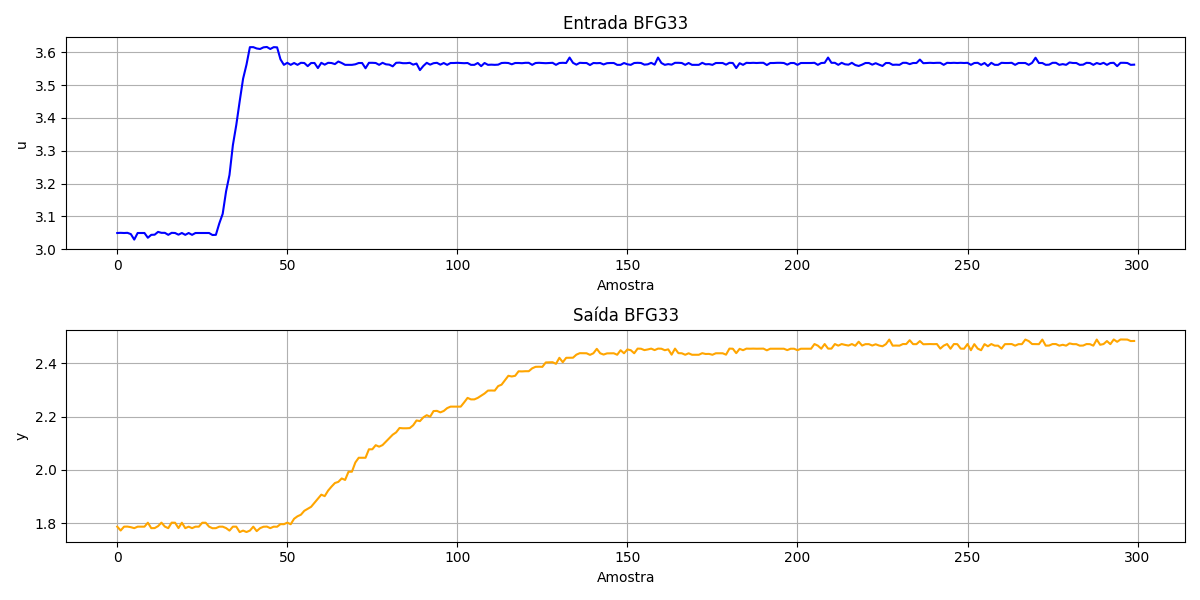
\includegraphics[width=0.8\textwidth]{imagens/bfg33_entrada_saida.png}
    \caption{Entrada e saída do sistema BFG33}
    \label{fig:bfg33_entrada_saida}
\end{figure}

A figura \ref{fig:bfg33_saida_estimada} mostra a saída estimada pelo modelo ARX para o sistema BFG33.

\begin{figure}[H]
    \centering
    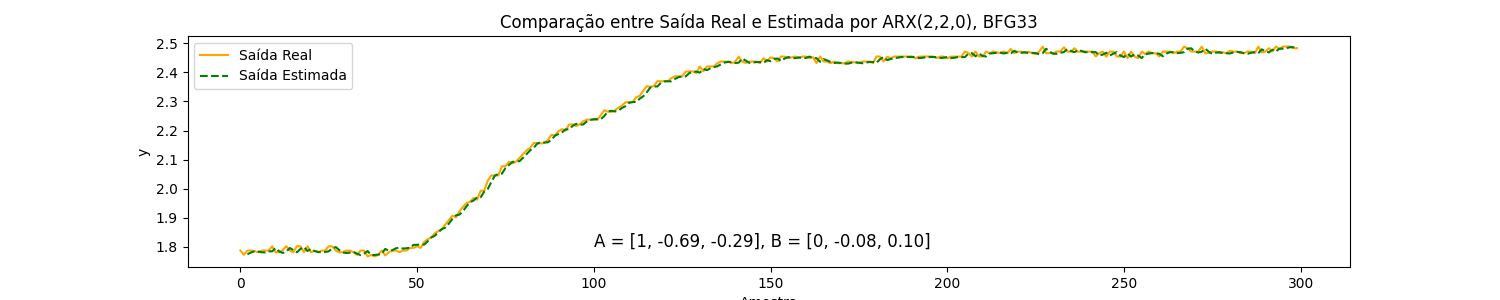
\includegraphics[width=0.8\textwidth]{imagens/bfg33_saida_estimada.png}
    \caption{Saída estimada pelo modelo ARX para o sistema BFG33}
    \label{fig:bfg33_saida_estimada}
\end{figure}

A figura \ref{fig:bfg33_nuvem_saidas} mostra a nuvem de curvas composta pelas saídas estimadas por 100 amostras da distribuição de parâmetros estimada para o modelo ARX do sistema BFG33.

\begin{figure}[H]
    \centering
    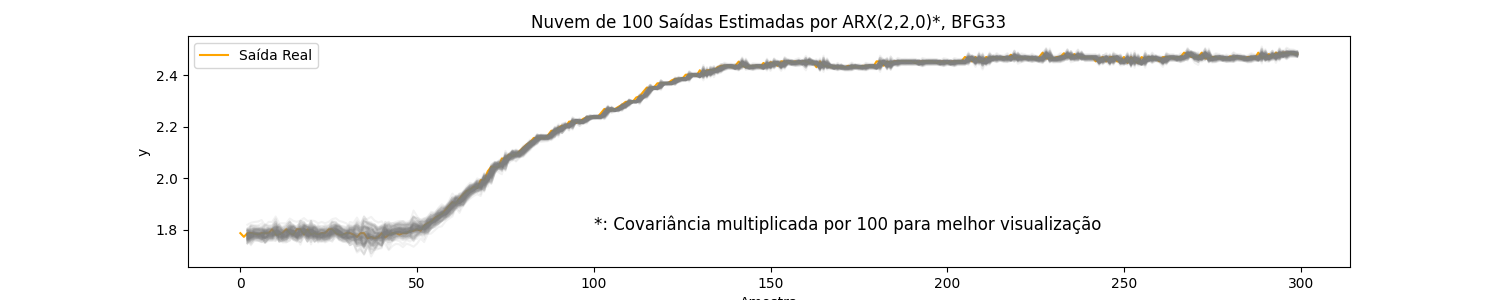
\includegraphics[width=0.8\textwidth]{imagens/bfg33_nuvem_saidas.png}
    \caption{Nuvem de curvas composta pelas saídas estimadas por 100 amostras da distribuição de parâmetros estimada para o modelo ARX do sistema BFG33}
    \label{fig:bfg33_nuvem_saidas}
\end{figure}

\subsection*{BFG44}

A figura \ref{fig:bfg44_entrada_saida} mostra o par de entrada e saída do sistema BFG44.

\begin{figure}[H]
    \centering
    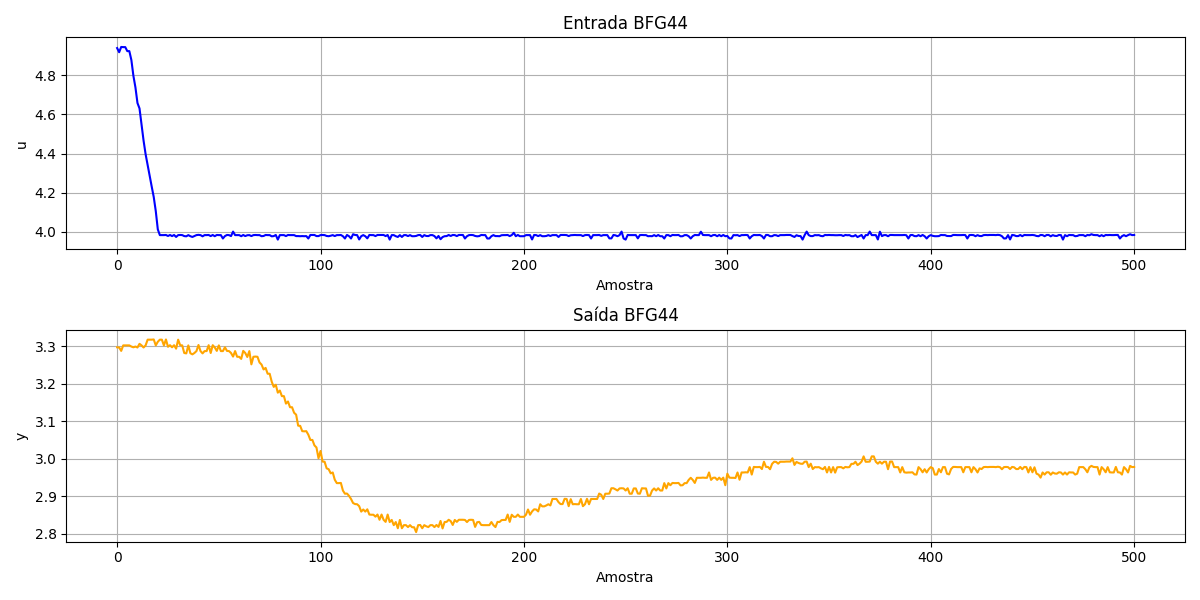
\includegraphics[width=0.8\textwidth]{imagens/bfg44_entrada_saida.png}
    \caption{Entrada e saída do sistema BFG44}
    \label{fig:bfg44_entrada_saida}
\end{figure}

A figura \ref{fig:bfg44_saida_estimada} mostra a saída estimada pelo modelo ARX para o sistema BFG44.

\begin{figure}[H]
    \centering
    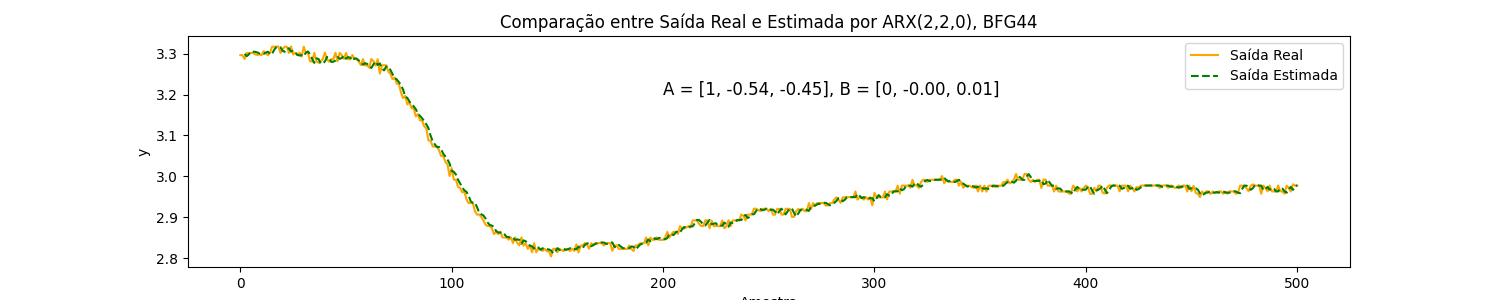
\includegraphics[width=0.8\textwidth]{imagens/bfg44_saida_estimada.png}
    \caption{Saída estimada pelo modelo ARX para o sistema BFG44}
    \label{fig:bfg44_saida_estimada}
\end{figure}

A figura \ref{fig:bfg44_nuvem_saidas} mostra a nuvem de curvas composta pelas saídas estimadas por 100 amostras da distribuição de parâmetros estimada para o modelo ARX do sistema BFG44.

\begin{figure}[H]
    \centering
    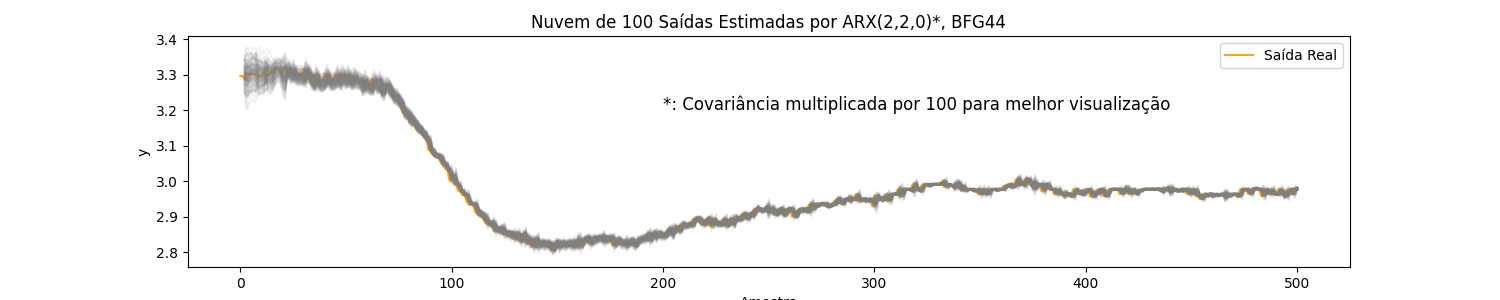
\includegraphics[width=0.8\textwidth]{imagens/bfg44_nuvem_saidas.png}
    \caption{Nuvem de curvas composta pelas saídas estimadas por 100 amostras da distribuição de parâmetros estimada para o modelo ARX do sistema BFG44}
    \label{fig:bfg44_nuvem_saidas}
\end{figure}

\end{document}
